\documentclass[12pt]{article} % A4 paper

\usepackage[T1]{fontenc} % Use 8-bit encoding that has 256 glyphs
\usepackage[utf8]{inputenc}

\usepackage[spanish, es-tabla]{babel} % Selecciona el español para palabras introducidas automáticamente, p.ej. "septiembre" en la fecha y especifica que se use la palabra Tabla en vez de Cuadro
\usepackage{graphics,graphicx, float} %para incluir imágenes y colocarlas
\usepackage{booktabs}
\usepackage{xcolor}

\parskip=3pt

\usepackage[
    a4paper,
    left=2.8cm,
    right=2.7cm,
    top=2.5cm,
    bottom=2.5cm
]{geometry}

\par

%----------------------------------------------------------------------------------------
%	TÍTULO Y DATOS DEL ALUMNO
%----------------------------------------------------------------------------------------

\title{	

\vspace{-2.5cm}
\LARGE \textbf{Técnicas de los Sistemas Inteligentes} \\
\LARGE Práctica 3: Satisfacción de restricciones con MiniZinc \\[0.5em]
\large Curso 2021-2022 \par
\large Pedro Bedmar López - 75935296Z \\
\normalsize pedrobedmar@correo.ugr.es \par
\large Grado en Ingeniería Informática
\vspace{-7pt}
\rule{\textwidth}{0.4pt}
\vspace{-2cm}
}

\date{}

%----------------------------------------------------------------------------------------
% DOCUMENTO
%----------------------------------------------------------------------------------------

\begin{document}

\clearpage
\maketitle % Muestra el Título

\section{Problema de las monedas}
En este ejercicio se pretende resolver el problema de que dada una cantidad de dinero, se devuelve en monedas de 1, 2, 5, 10, 20 y 50 céntimos y en monedas de 1 y 2 euros.

De por sí, el encontrar una única solución al problema de las monedas se engloba en la clase de problemas NP-completos. Esto se debe a que:
\begin{itemize}
    \item SAT $\leq_P$ Coin-Problem: Existe una reducción en tiempo polinomial desde este problema a otro que ya se ha demostrado que pertenece a la clase NP-completo, como es SAT.
    \item Dada una posible solución al problema de las monedas, se puede verificar si es válida o no en tiempo polinomial.
\end{itemize}
Estamos ante lo que se conoce como un problema de decisión.

\subsection{Apartado a)}

En los apartados a y b no se nos pide encontrar una única solución: se nos pide conocer todas las soluciones posibles. Por ello, nos encontramos ante un problema que tiene una complejidad mayor que encontrar una única solución.

Encontrarlas todas no es un problema NP-completo, sino NP-duro. Dada una lista de posibles soluciones, no podemos verificar en tiempo polinomial si esas son todas las existentes. Otra forma de verlo es dándose cuenta de que no estamos ante un problema de decisión. Por tanto, no estamos ante un problema NP-completo.

Como se puede observar en la siguiente tabla, el número de soluciones crece muy rápidamente (y de la misma forma lo hace el tiempo de ejecución). En cada uno de los cuatro casos, la solución encontrada se expresa como un vector [c1,c2,c5,c10,c20,c50,e1,e2], donde cx representa la cantidad de monedas de x céntimos y ex la cantidad de monedas de x euros.

\begin{table}[H]
\centering
\begin{tabular}{@{}c|lll@{}}
\toprule
Importe &
    \multicolumn{1}{c}{\begin{tabular}[c]{@{}c@{}}Primera solución encontrada\\ y número de monedas de la misma\end{tabular}} &
    \multicolumn{1}{c}{\begin{tabular}[c]{@{}c@{}}Número total\\ de soluciones\end{tabular}} &
    \multicolumn{1}{c}{\begin{tabular}[c]{@{}c@{}}Runtime\\ (en segundos)\end{tabular}} \\ \midrule
0.17€ & {[}17,0,0,0,0,0,0,0{]} $\rightarrow$ 17 monedas   & 28     & 0.286  \\
1.43€ & {[}143,0,0,0,0,0,0,0{]} $\rightarrow$ 143 monedas & 17952  & 2.692  \\
2.35€ & {[}235,0,0,0,0,0,0,0{]} $\rightarrow$ 235 monedas & 150824 & 25.764 \\
4.99€ & {[}499,0,0,0,0,0,0,0{]} $\rightarrow$ 499 monedas & 6224452  & 2002 \\ \bottomrule
\end{tabular}
\caption{Resultados del apartado a) del problema de las monedas.}
\label{tab:my-table}
\end{table}

\subsection{Apartado b)}
En este caso, añadimos restricciones extra que impiden que con monedas de céntimo podamos representar un euro o más. Debido a esto, el espacio de búsqueda se va a reducir y el tiempo de ejecución por tanto también disminuye. 

\begin{table}[H]
\centering
\begin{tabular}{@{}c|lll@{}}
\toprule
Importe &
    \multicolumn{1}{c}{\begin{tabular}[c]{@{}c@{}}Primera solución encontrada\\ y número de monedas de la misma\end{tabular}} &
    \multicolumn{1}{c}{\begin{tabular}[c]{@{}c@{}}Número total\\ de soluciones\end{tabular}} &
    \multicolumn{1}{c}{\begin{tabular}[c]{@{}c@{}}Runtime\\ (en segundos)\end{tabular}} \\ \midrule
0.17€ & {[}17,0,0,0,0,0,0,0{]} $\rightarrow$ 17 monedas  & 28    & 0.342 \\
1.43€ & {[}43,0,0,0,0,0,1,0{]} $\rightarrow$ 44 monedas & 284   & 0.311 \\
2.35€ & {[}35,0,0,0,0,0,2,0{]} $\rightarrow$ 37 monedas & 324   & 0.412 \\
4.99€ & {[}99,0,0,0,0,0,4,0{]} $\rightarrow$ 103 monedas & 13098 & 2.200 \\ \bottomrule
\end{tabular}
\caption{Resultados del apartado b) del problema de las monedas}
\label{tab:my-table}
\end{table}

\subsection{Apartado c)}
En este caso observamos que los tiempos de ejecución son menores o iguales que en el caso anterior. Esto se debe a que para problemas de optimización, MiniZinc no recorre todo el espacio de búsqueda: al inicio, elige una solución cualquiera y entra en un proceso iterativo donde añade como restricción que la próxima solución tenga un coste inferior a la actual. Esto se repite hasta que se encuentra con un problema insatisfacible. En ese momento sabe que la solución óptima es la generada en el paso anterior y es la que se devuelve.

Esto permite acotar en gran medida la búsqueda y acelerar el proceso, como se observa en la tabla inferior.
% TODO: es correcto?

% Please add the following required packages to your document preamble:
% \usepackage{booktabs}
\begin{table}[H]
    \centering
    \begin{tabular}{@{}c|ll@{}}
    \toprule
    Importe &
      \multicolumn{1}{c}{\begin{tabular}[c]{@{}c@{}}Solución óptima y número\\ de monedas de la misma\end{tabular}} &
      \multicolumn{1}{c}{\begin{tabular}[c]{@{}c@{}}Runtime\\ (en segundos)\end{tabular}} \\ \midrule
    0.17\texteuro  & {[}0,1,1,1,0,0,0,0{]} $\rightarrow$ 3 monedas & 0.283 \\
    1.43\texteuro  & {[}1,1,0,0,2,0,1,0{]} $\rightarrow$ 5 monedas & 0.327 \\
    2.35\texteuro  & {[}0,0,1,1,1,0,0,1{]} $\rightarrow$ 4 monedas & 0.338 \\
    4.99\texteuro  & {[}0,2,1,0,2,1,0,2{]} $\rightarrow$ 8 monedas & 0.376 \\ \bottomrule
    \end{tabular}
    \caption{Resultados del apartado c) del problema de las monedas}
    \label{tab:my-table}
    \end{table}

\subsection{Apartado d)}
\subsubsection*{¿Qué ocurriría si, usando la codificación (a) para encontrar todas las soluciones, el importe buscado es mucho mayor?} 

Como hemos mencionado anteriormente, este problema es NP-duro.

Ocurre que el espacio de búsqueda crece exponencialmente, y de la misma forma lo hace el tiempo de ejecución, por lo tanto llega un punto en el que el problema es inabarcable. 

\subsubsection*{¿Se podría encontrar alguna solución (usando la codificación de (a) o cualquier otra) de este problema con un importe del orden de los millones de euros? En caso afirmativo, ¿cuál podría ser una estrategia prometedora?}
Sí, una codificación donde únicamente existan monedas de un céntimo podría resolver el problema con tiempos de ejecución menores. En cada iteración, hasta llegar a la cantidad deseada, se aumentaría una variable contador en un céntimo. Su coste computacional sería O(n), donde n es el número de céntimos de la cantidad a alcanzar.

Otra estrategia aún más prometedora escogería primero las monedas más grandes posibles. En el momento en el que esa moneda tiene un valor mayor que el dinero restante, se utiliza la siguiente moneda y así sucesivamente. De esta forma minimizamos el número de monedas necesarias y se reduce el espacio de búsqueda.
%TODO: Está correcto lo que acabo de explicar?

\section{Problema de los horarios}
Como se puede observar en las tablas inferiores, existen dos soluciones para este problema. La única diferencia entre ellas es el intercambio de las asignaturas en color rojo.

\begin{table}[H]
\centering
\begin{tabular}{c|ccccc}
\multicolumn{1}{l|}{} & L  & M  & X  & J  & V  \\ \hline
8-9                   & A4 & A4 & A8 & A5 & A5 \\
9-10                  & A4 & A4 & A8 & A5 & A5 \\
10-11                 & A9 & A7 & A6 & A2 & A6 \\
11-12                 & NA & NA & NA & NA & NA \\
12-13                 & A1 & A1 & A3 & A3 & \color{red}A2 \\
13-14                 & A1 & A1 & A3 & A3 & \color{red}A7
\end{tabular}
\caption{Solución 1 al problema de los horarios}
\label{tab:my-table}
\end{table}
\vspace{2pt}
\begin{table}[H]
\centering
\begin{tabular}{c|ccccc}
\multicolumn{1}{l|}{} & L  & M  & X  & J  & V  \\ \hline
8-9                   & A4 & A4 & A8 & A5 & A5 \\
9-10                  & A4 & A4 & A8 & A5 & A5 \\
10-11                 & A9 & A7 & A6 & A2 & A6 \\
11-12                 & NA & NA & NA & NA & NA \\
12-13                 & A1 & A1 & A3 & A3 & \color{red}A7 \\
13-14                 & A1 & A1 & A3 & A3 & \color{red}A2
\end{tabular}
\caption{Solución 2 al problema de los horarios}
\label{tab:my-table}
\end{table}

En mi caso, por cómo he representado el problema y por las restricciones que he empleado, no he obtenido soluciones simétricas. Un caso donde se me ocurre que podrían aparecer es utilizando identificadores distintos para cada recreo. En mi caso, los recreos siempre los fuerzo a tomar valor 0, pero si pudieran tomar valores diferentes para cada día (-1, -2, -3, -4 y -5, por ejemplo) aquí encontraríamos simetrías, soluciones que semánticamente significan lo mismo, pero que poseen valores diferentes. El recreo del lunes podría tomar valor -1 y el del martes -2, pero también podría ocurrir al revés, siendo las soluciones semánticamente idénticas.

Otra simetría aparecería si nuestra codificación diferenciara cada uno de los bloques lectivos de una misma asignatura. En ese caso, por ejemplo, las dos primeras horas del lunes y del martes se podrían intercambiar, dando lugar a dos soluciones semánticamente idénticas.

Como podemos observar, la estrategia para evitar simetrías consiste en hacer coincidir el dominio de las variables con su dominio semántico, de forma que la cardinalidad de ambos sea la misma.
% TODO: está esto bien?

\section{Problema lógico}
En este ejercicio solo existe una solución posible: el andaluz bebe agua y la cebra está en la casa verde.
% TODO: qué más poner en este ejercicio?

\section{Problema de la asignación de tareas}
A continuación mostramos los diagramas de Gantt con las soluciones óptimas al problema de asignación de tareas. El primer trabajador aparece representado por el color azul, el segundo trabajador por el rojo y el tercero por el verde.

Utilizando la primera versión del ejercicio, sin el cuarto trabajador de apoyo, el tiempo mínimo requerido para completar la construcción es de 12 días.

\begin{figure}[H] %con el [H] le obligamos a situar aquí la figura
    \centering
        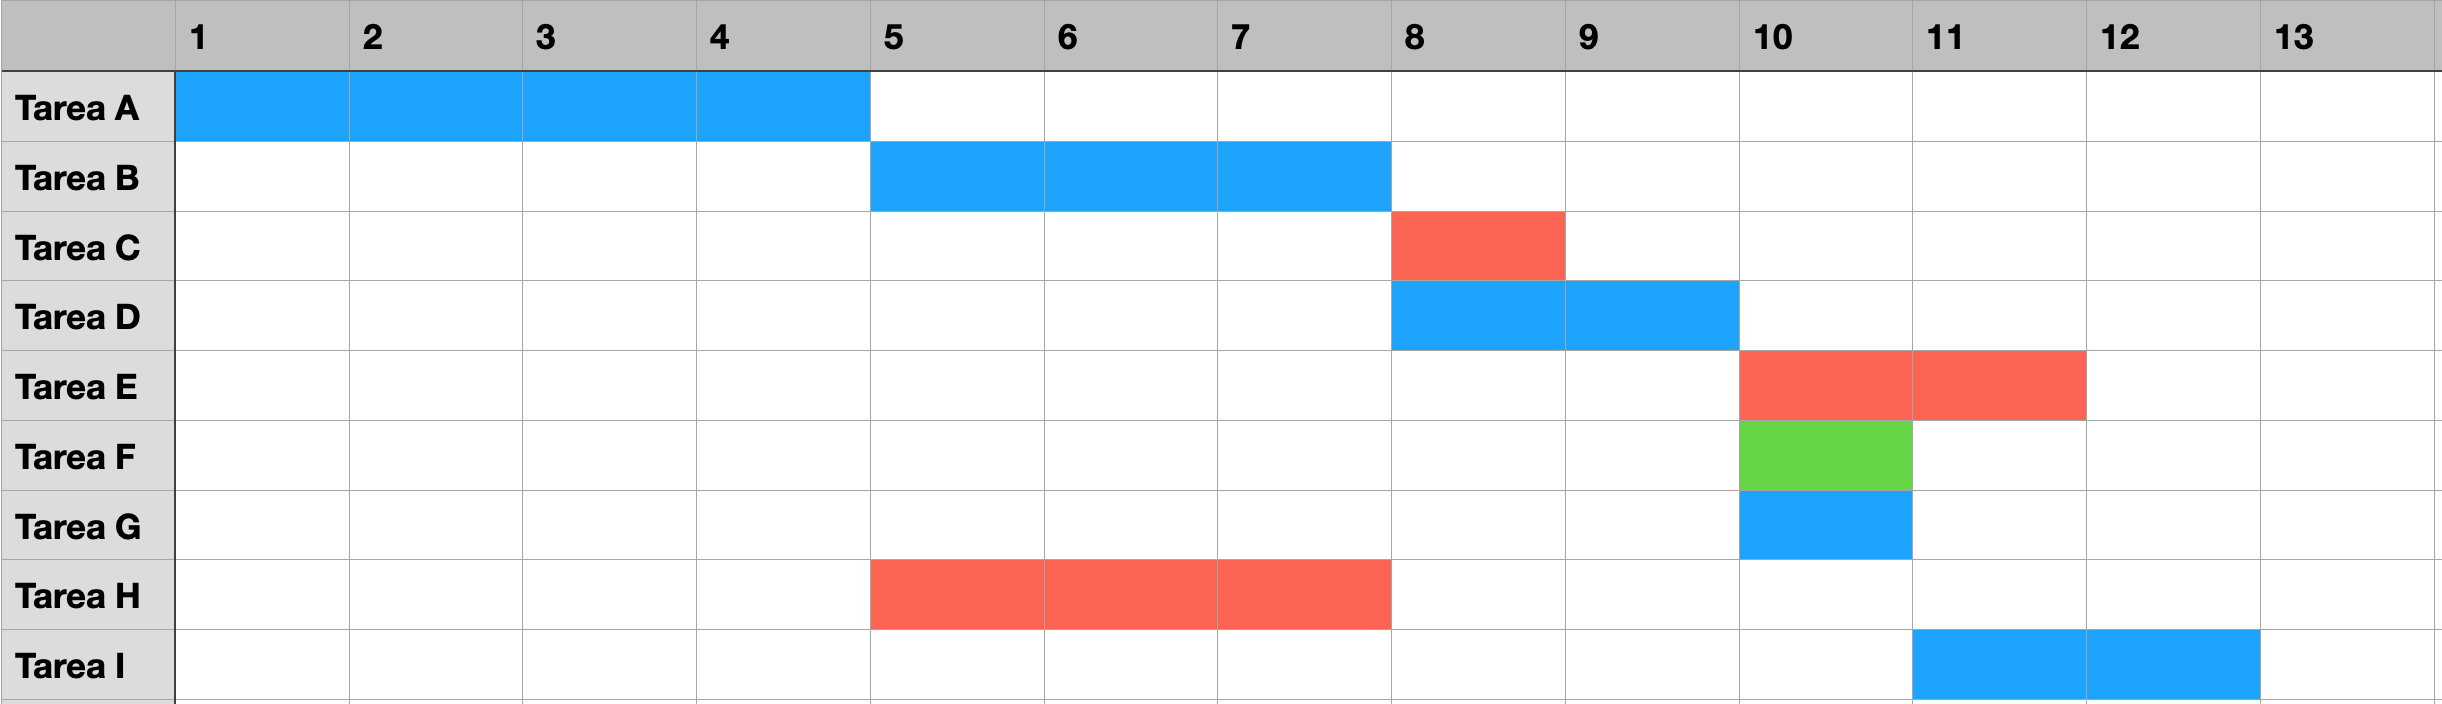
\includegraphics[scale=0.32]{gantt.png}
        \caption{Diagrama de Gantt de la solución sin el cuarto trabajador}
\end{figure}

En la segunda versión, este tiempo se reduce a 8 días. En las tareas que participa el trabajador de apoyo lo indicamos escribiendo T. extra.

\begin{figure}[H] %con el [H] le obligamos a situar aquí la figura
    \centering
        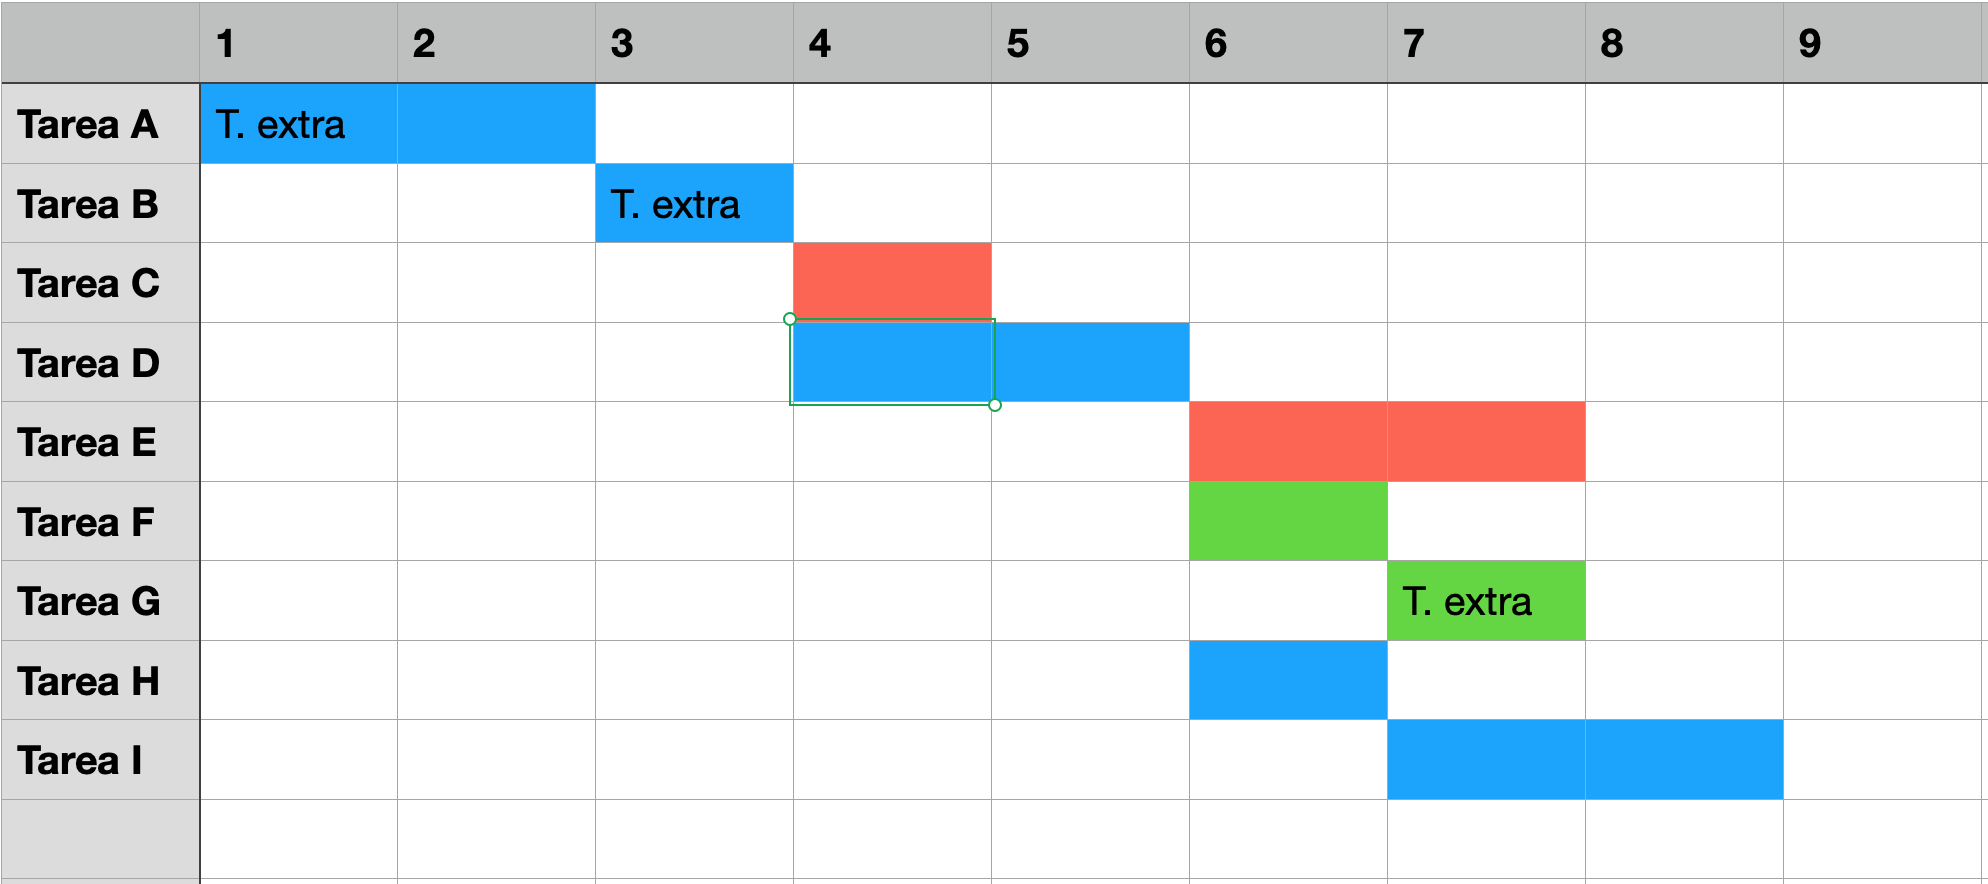
\includegraphics[scale=0.32]{gantt2.png}
        \caption{Diagrama de Gantt de la solución utilizando el trabajador adicional}
\end{figure}

\section{Problema del coloreado de grafos}
En la siguiente tabla se pueden apreciar los resultados de ejecución para diferentes tamaños de grafos. En cada caso, realizamos 3 ejecuciones y en la tabla indicamos el número de colores mínimo y tiempo de ejecución promedios. Para generar los grafos siempre utilizamos las mismas semillas: 0, 1 y 2.

\begin{table}[H]
\centering
\begin{tabular}{c|cc}
\multicolumn{1}{l|}{Tamaño del grafo} &
    \begin{tabular}[c]{@{}c@{}}Número de\\ colores mínimo\end{tabular} &
    \begin{tabular}[c]{@{}c@{}}Runtime\\ (en segundos)\end{tabular} \\ \hline
N=4, M=6   & 2.667   & 0.507 \\
N=6, M=15  & 4.667   & 0.554 \\
N=8, M=28  & 6.333   & 0.350 \\
N=10, M=45 & 8       & 2.473 \\
N=12, M=66 & 9       & 14.54  \\
N=14, M=91 & 11.333  & 2330.33    
\end{tabular}
\caption{Valores medios de ejecución del problema de coloreado de grafos}
\label{tab:my-table}
\end{table}

En respuesta a la pregunta formulada en el guion, no es un problema que pueda escalar de forma sencilla, debido a que es NP-duro. Existe una reducción de este problema a MAXSAT: MAXSAT $\leq_P$ Edge-Coloring.

Es NP-duro pero no se encuentra en NP, por lo tanto no es NP-completo. Esto es así porque no es un problema de decisión, sino de optimización. Otra forma de comprobar lo mismo es observando que dada una posible solución del problema, no podemos verificar si es la óptima en tiempo polinomial.

Los problemas NP-duros se pueden resolver en tiempo polinomial por una máquina de Turing no determinista. Aunque se cree que no existen algoritmos que permiten ejecutarlos en tiempo polinomial en una máquina determinista, no se ha demostrado formalmente.

Es por ello que son problemas muy costosos y no escalan de forma adecuada.

\end{document}